%%%%%%%%%%%%%%%%%%%%%%%%%%%%%%%%%%%%%%%%
\section{Confronto del modello predefinito e ottimizzato}
Con l'ottimizzazione effettuata nel paragrafo precedente si è andati a effettuare un confronto tra il modello appena ottimizzato e il modello predefinito, utilizzando grafici analoghi a quelli riportati nella \autoref{ch:default}.
Andando a osservare lo spettro di produzione di $p+\bar p$ non dovremmo osservare particolare differenze, come nel modello pedefinito.
Infatti, come visibile in \autoref{fig:D_pp}, osserviamo un andamento praticamente identico a quello di \autoref{fig:A_pp}.
\begin{figure}[htb]
    \centering
    \begin{subfigure}{.49\textwidth}
    \centering
        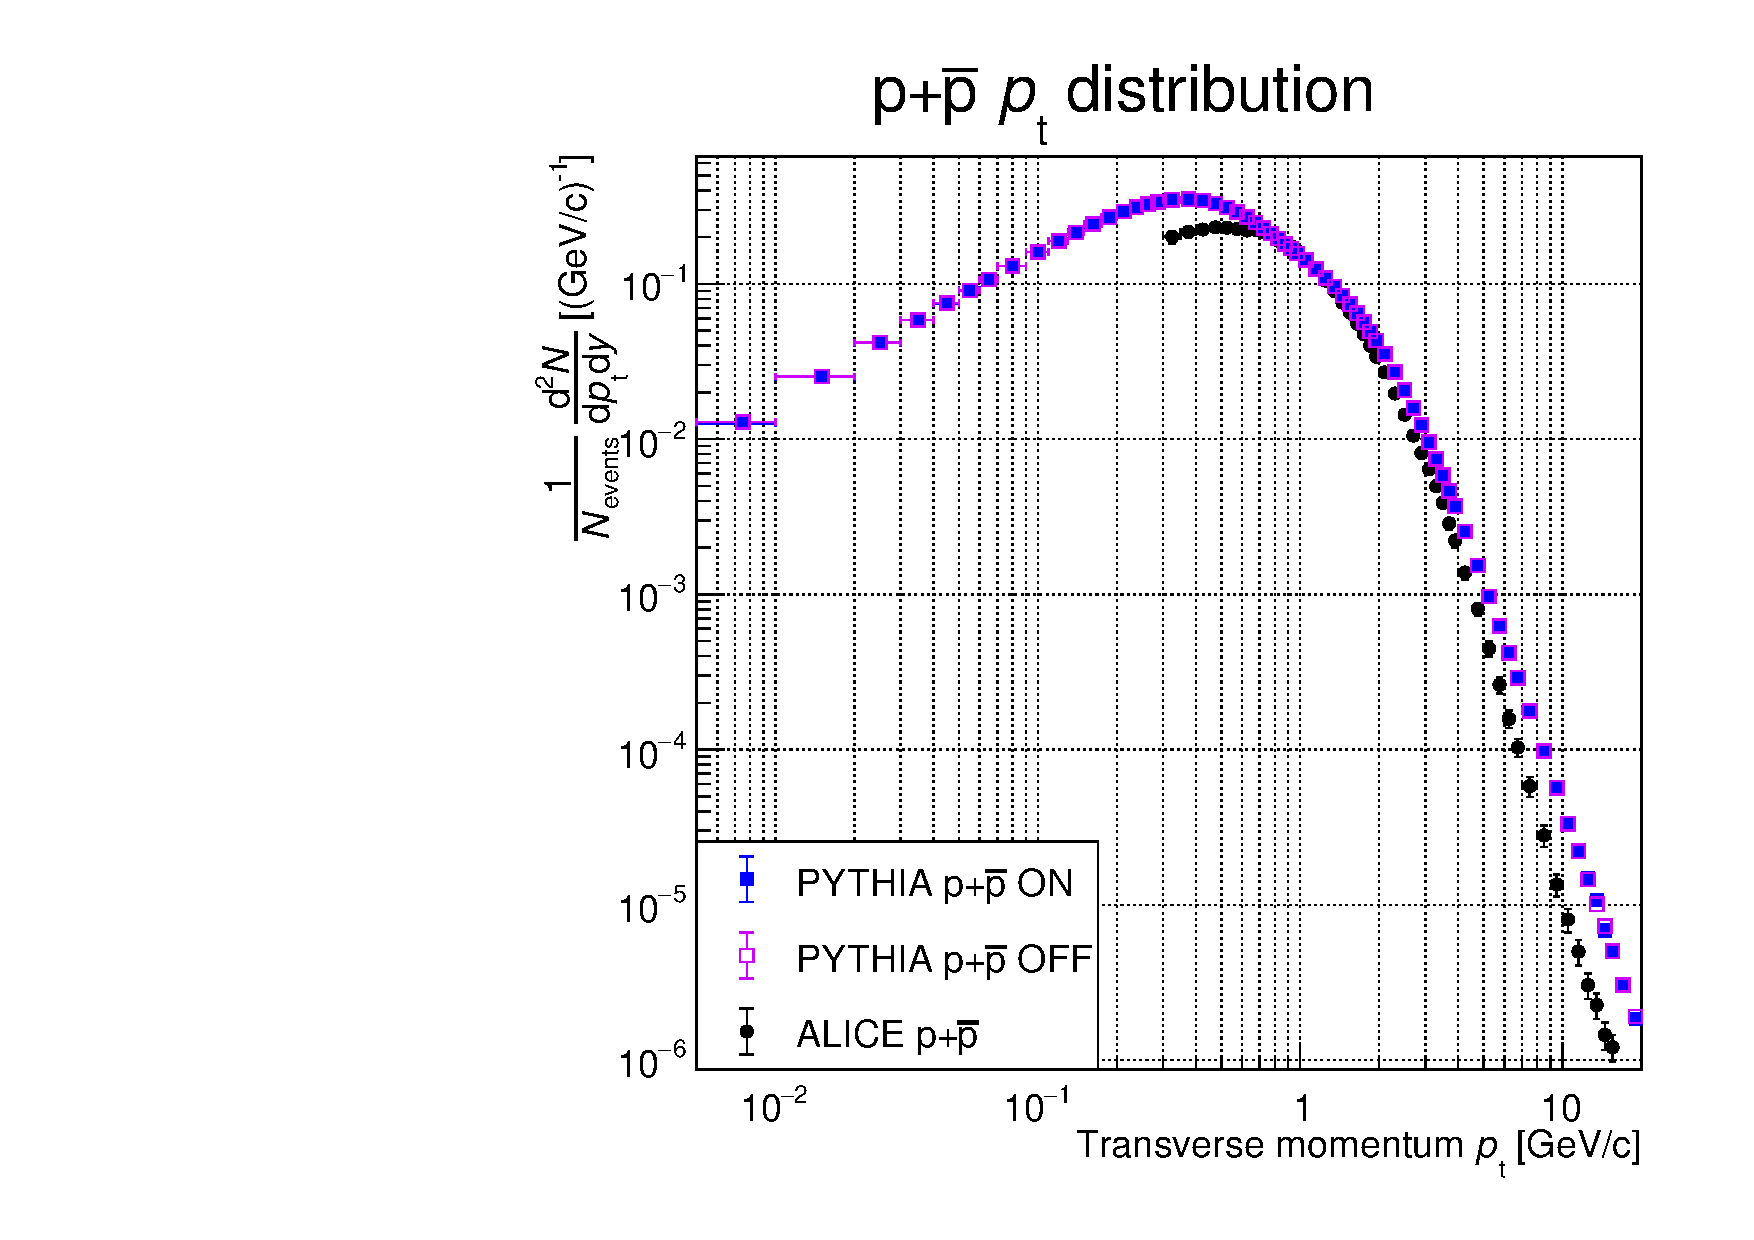
\includegraphics[width=\textwidth]{image/3-risultati/analyse/G/pp.pdf}
        \caption{}
        \label{fig:D_pp}
    \end{subfigure}
    %\hspace{1cm}
    \begin{subfigure}{.49\textwidth}
        \centering
        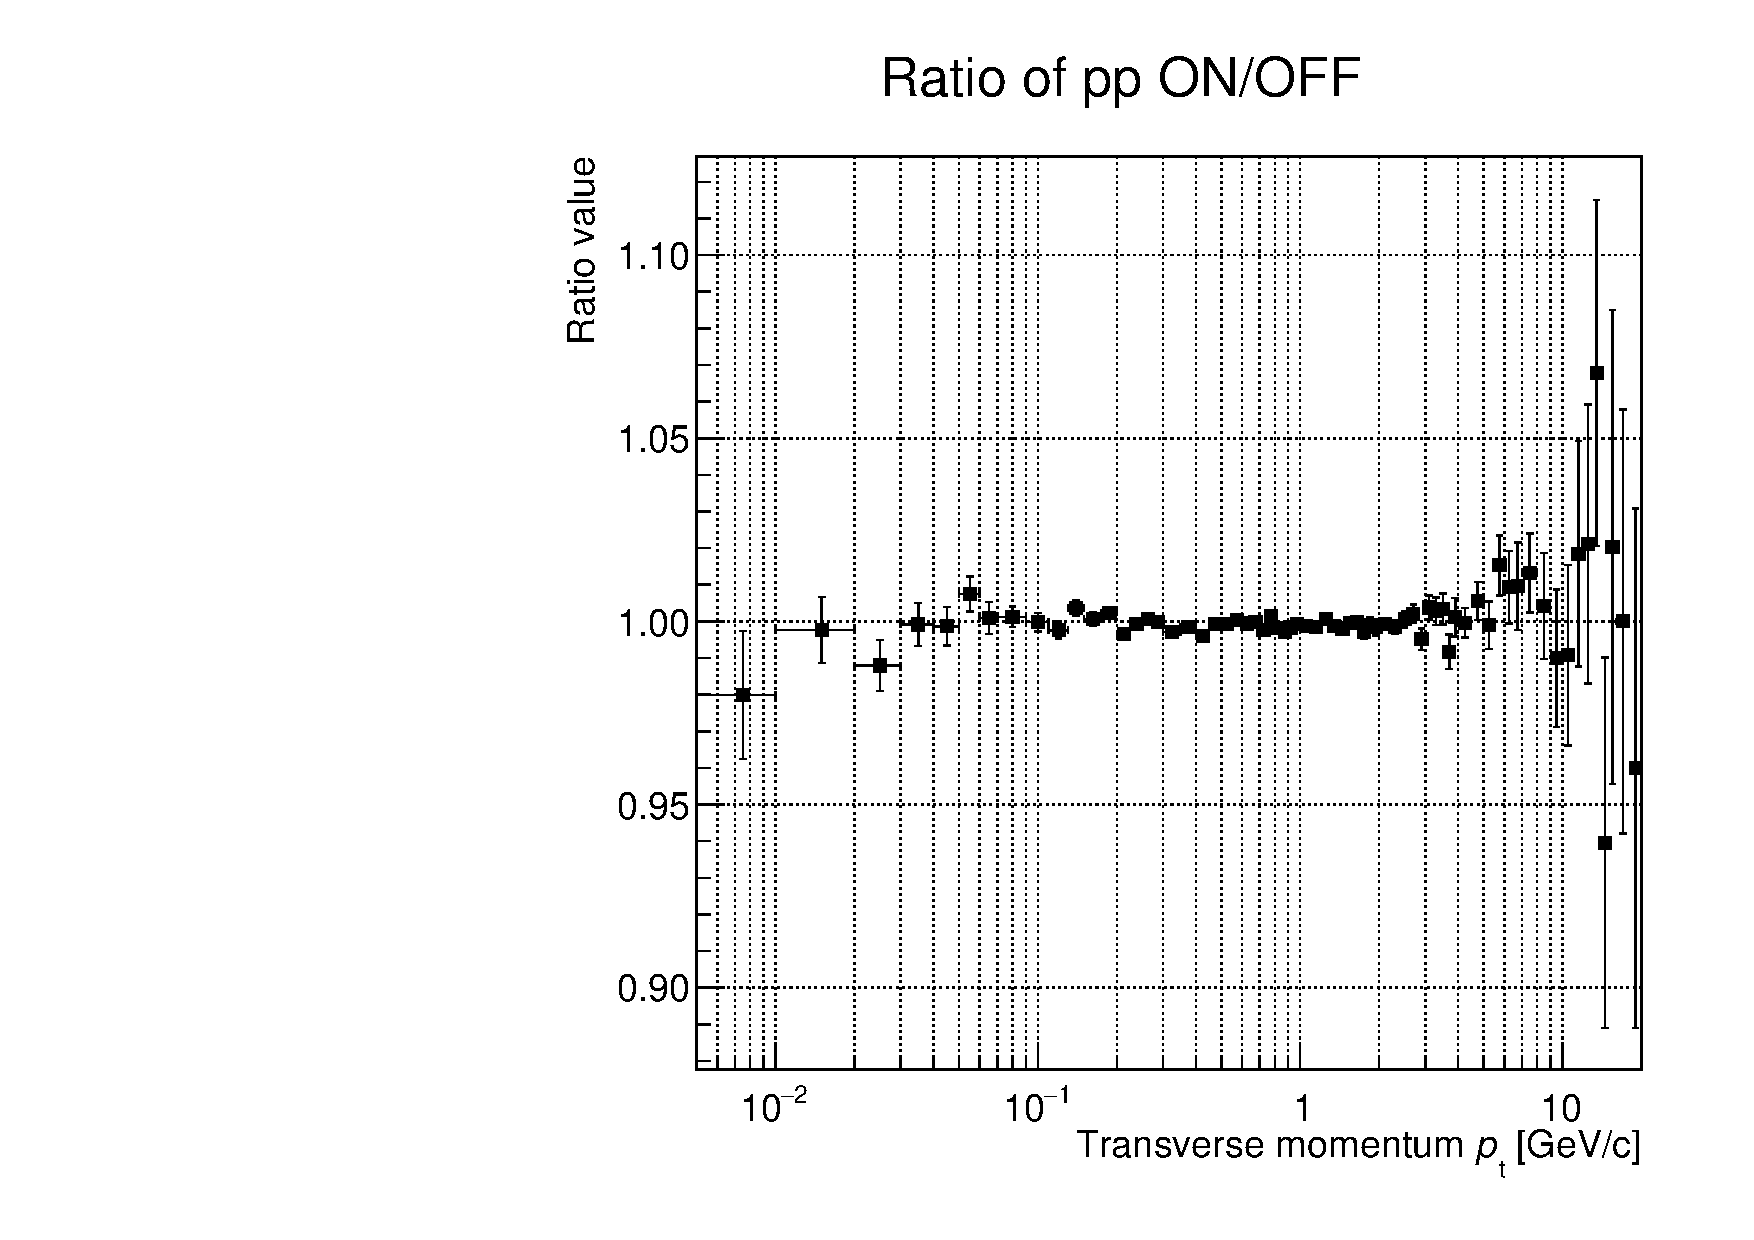
\includegraphics[width=\textwidth]{image/3-risultati/analyse/G/ratio_pp_ON_OFF.pdf}
        \caption{}
        \label{fig:D_ratio_pp_ON_OFF}
    \end{subfigure}
    \captionwithsource{\emph{\rmfamily (a)} Distribuzione dell'impulso trasverso di $p+\bar p$ con produzione deuteronica attivata e disattivata ("ON" e "OFF") in confronto con i dati sperimentali di ALICE ("ALICE"), usando il modello ottimizzato. \emph{\rmfamily (b)} Frazione della distribuzione dell'impulso trasverso di $p+\bar p$ con produzione deuteronica attivata e con produzione non attivata, usando il modello ottimizzato.}{\cite{ALICE:2020jsh}}
    \label{fig:D_pp_prod}
\end{figure}
Neanche il rapporto tra il caso in cui la produzione deuteronica sia attivata e quella disattivata presenta particolari differenze, come si può notare in \autoref{fig:D_ratio_pp_ON_OFF}, con un valore della media pesata di $0.99889 \pm 0.00024$, vicino al valore di 0.999.

Per quanto riguarda gli spettri dei (anti)deuteroni (in \autoref{fig:D_(anti)deuteron}) essi mostrano un accordo migliore con i dati rispetto al modello predefinito, come si può osservare in \autoref{fig:A_(anti)deuteron}.
Ciò è supportato andando a effettuare una divisione tra i dati dei (anti)deuteroni di \pythia{} e di ALICE ottenendo così il grafico riportato in \autoref{fig:D_division}.
Come già anticipato, il valore della media pesata del rapporto è di $1.0467 \pm 0.015$ per i deuteroni e $ 0.968 \pm 0.021$ per gli antideuteroni, più vicini al valore unitario rispetto a quello del modello predefinito.

Anche qui si esegue una verifica della correttezza delle simulazioni andando a vedere il bilancio deuteroni-antideuteroni.
Effettuando una divisione tra gli istogrammi dei deuteroni e degli antideuteroni (\autoref{fig:D_ratio_DD}), si ottiene un valore della media pesata di $1.017 \pm 0.008$, compatibile entro 3 sigma con il valore unitario.\\

Per ultimo si esegue un confronto tra i due modelli.
Si ottiene il grafico visibile in \autoref{fig:def_opt}.
È importante notare come le distribuzioni di produzione di (anti)deuterone in funzione dell'impulso trasverso ottenute con i due modelli abbiano in realtà lo stesso identico andamento ma valori assoluti diversi; ciò è dovuto al fatto che le variazioni del parametro \ttbox{norm} agiscono sul numero complessivo di (anti)deuteroni prodotti in tutti i canali di produzione.
Gli spettri prodotti hanno quindi la medesima forma ma un differente fattore di scala.
\begin{figure}[htp]
    \centering
    \begin{subfigure}{.49\textwidth}
    \centering
        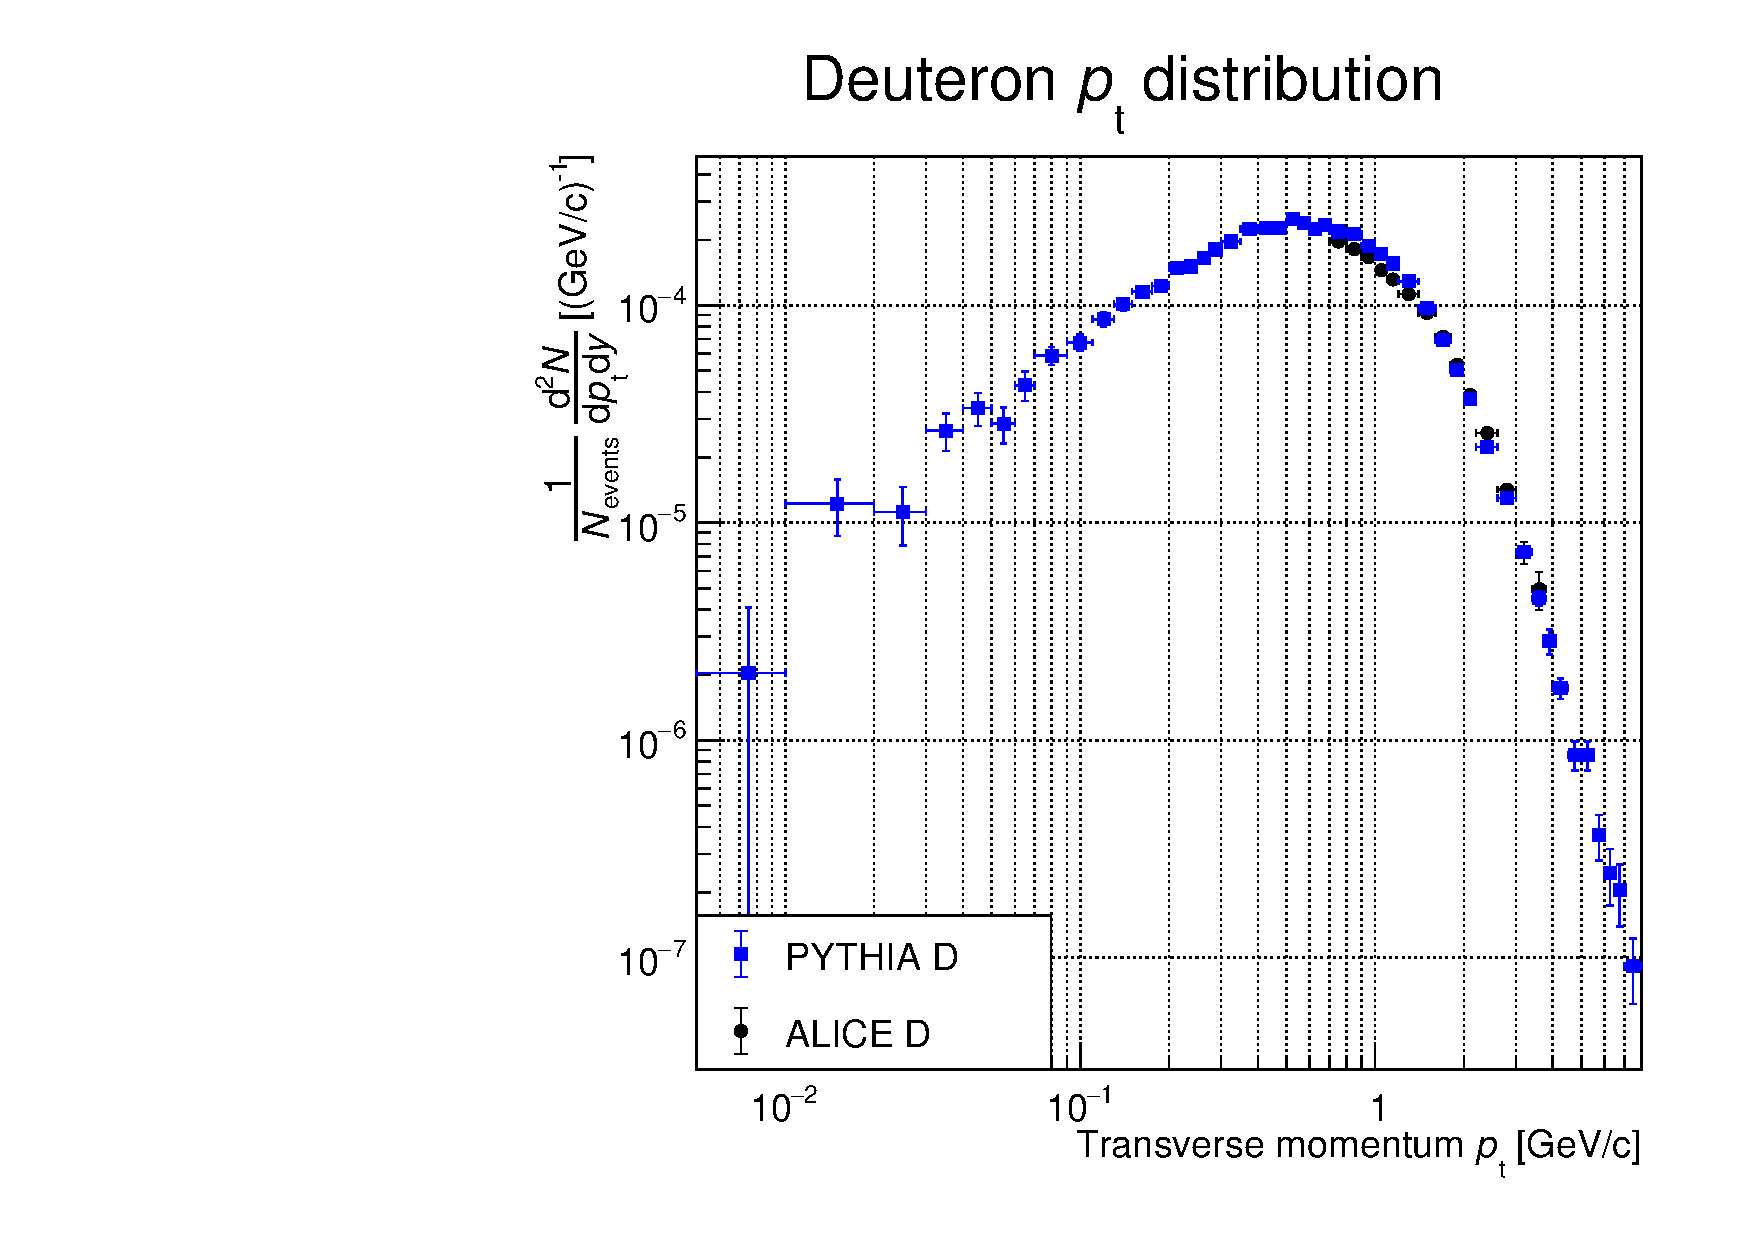
\includegraphics[width=\textwidth]{image/3-risultati/analyse/G/deuteron.pdf}
        \caption{}
        \label{fig:D_deuteron}
    \end{subfigure}
    %\hspace{1cm}
    \begin{subfigure}{.49\textwidth}
        \centering
        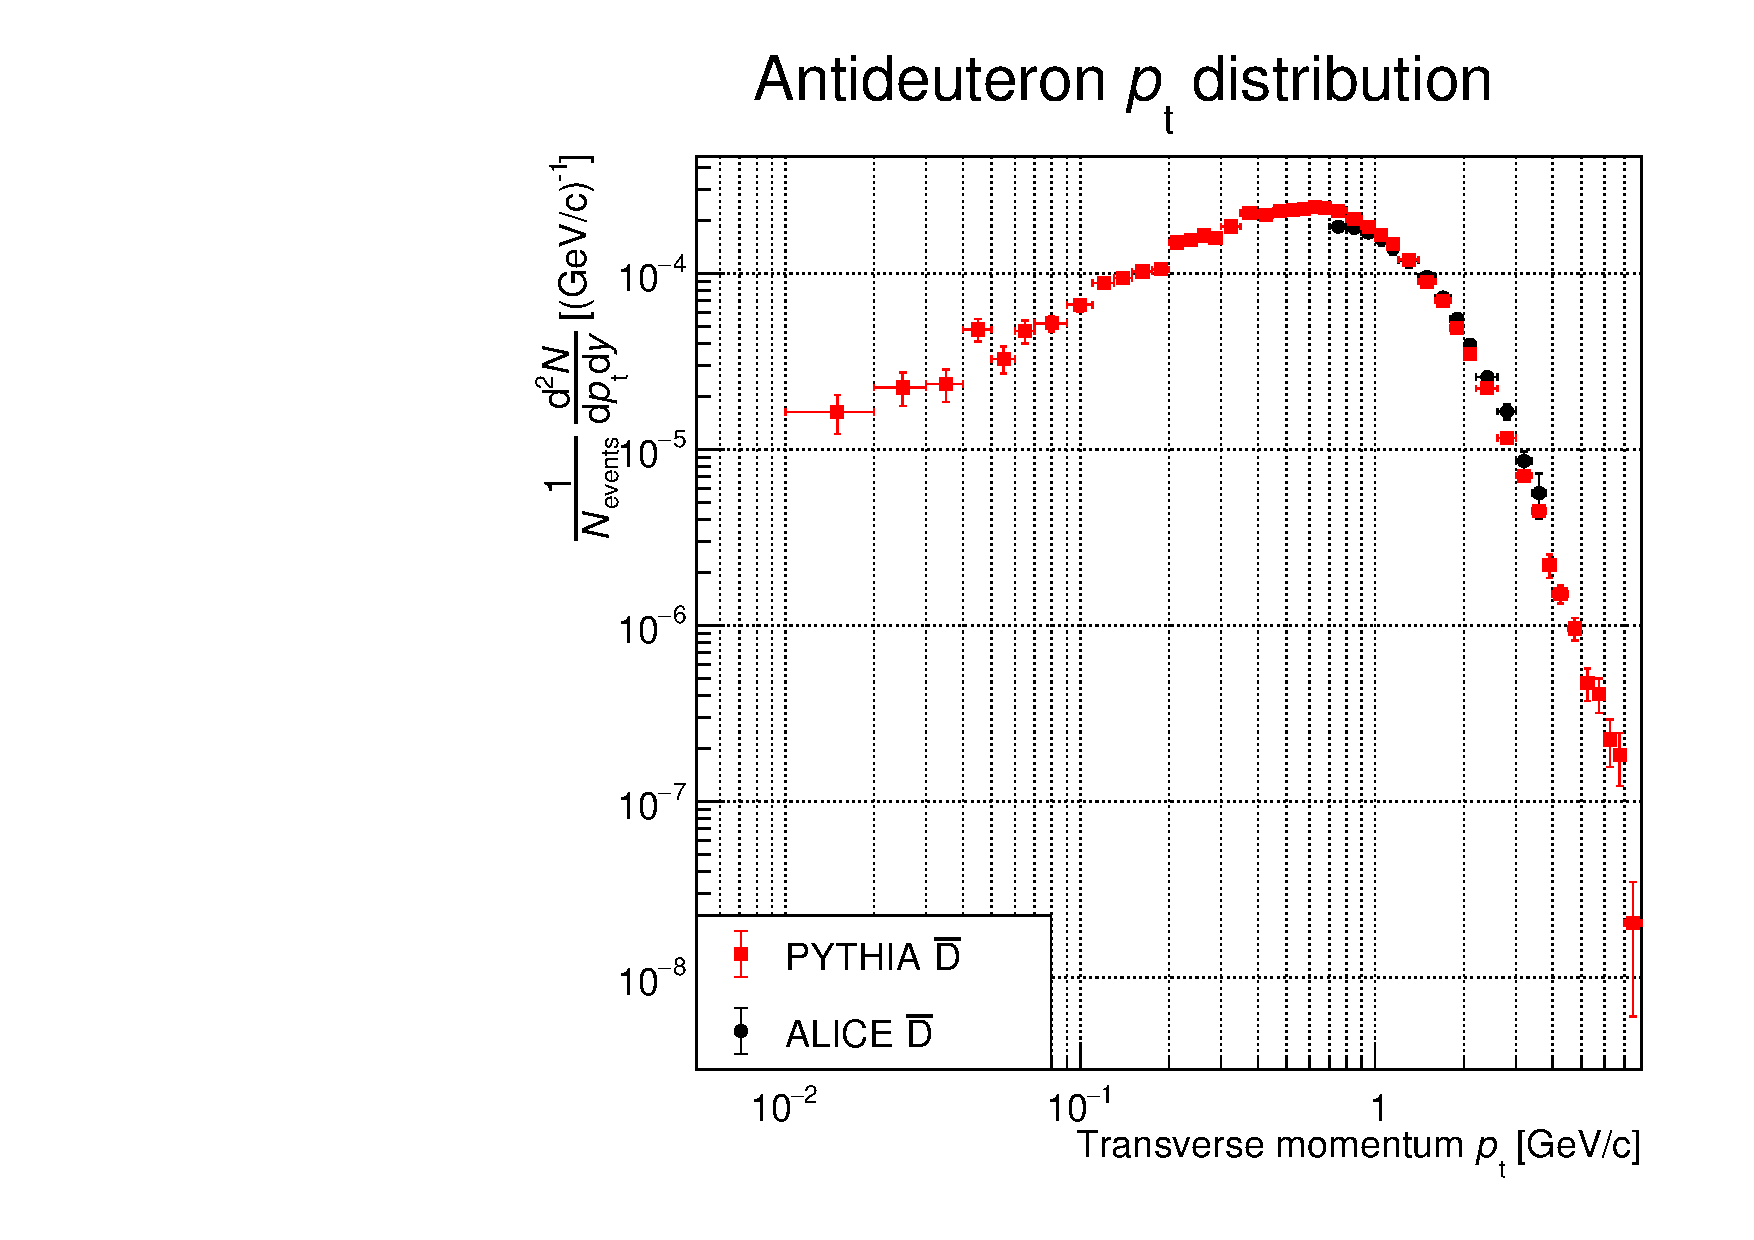
\includegraphics[width=\textwidth]{image/3-risultati/analyse/G/antideuteron.pdf}
        \caption{}
        \label{fig:D_antideuteron}
    \end{subfigure}
    \captionwithsource{Distribuzione dell'impulso trasverso di \emph{\rmfamily (a)} $D$ e \emph{\rmfamily (b)} di $\bar D$ in confronto con i dati di ALICE, utilizzando il modello ottimizzato.}{\cite{ALICE:2020foi}}
    \label{fig:D_(anti)deuteron}
\end{figure}
\begin{figure}[htp]
    \centering
    \begin{subfigure}{.49\textwidth}
    \centering
        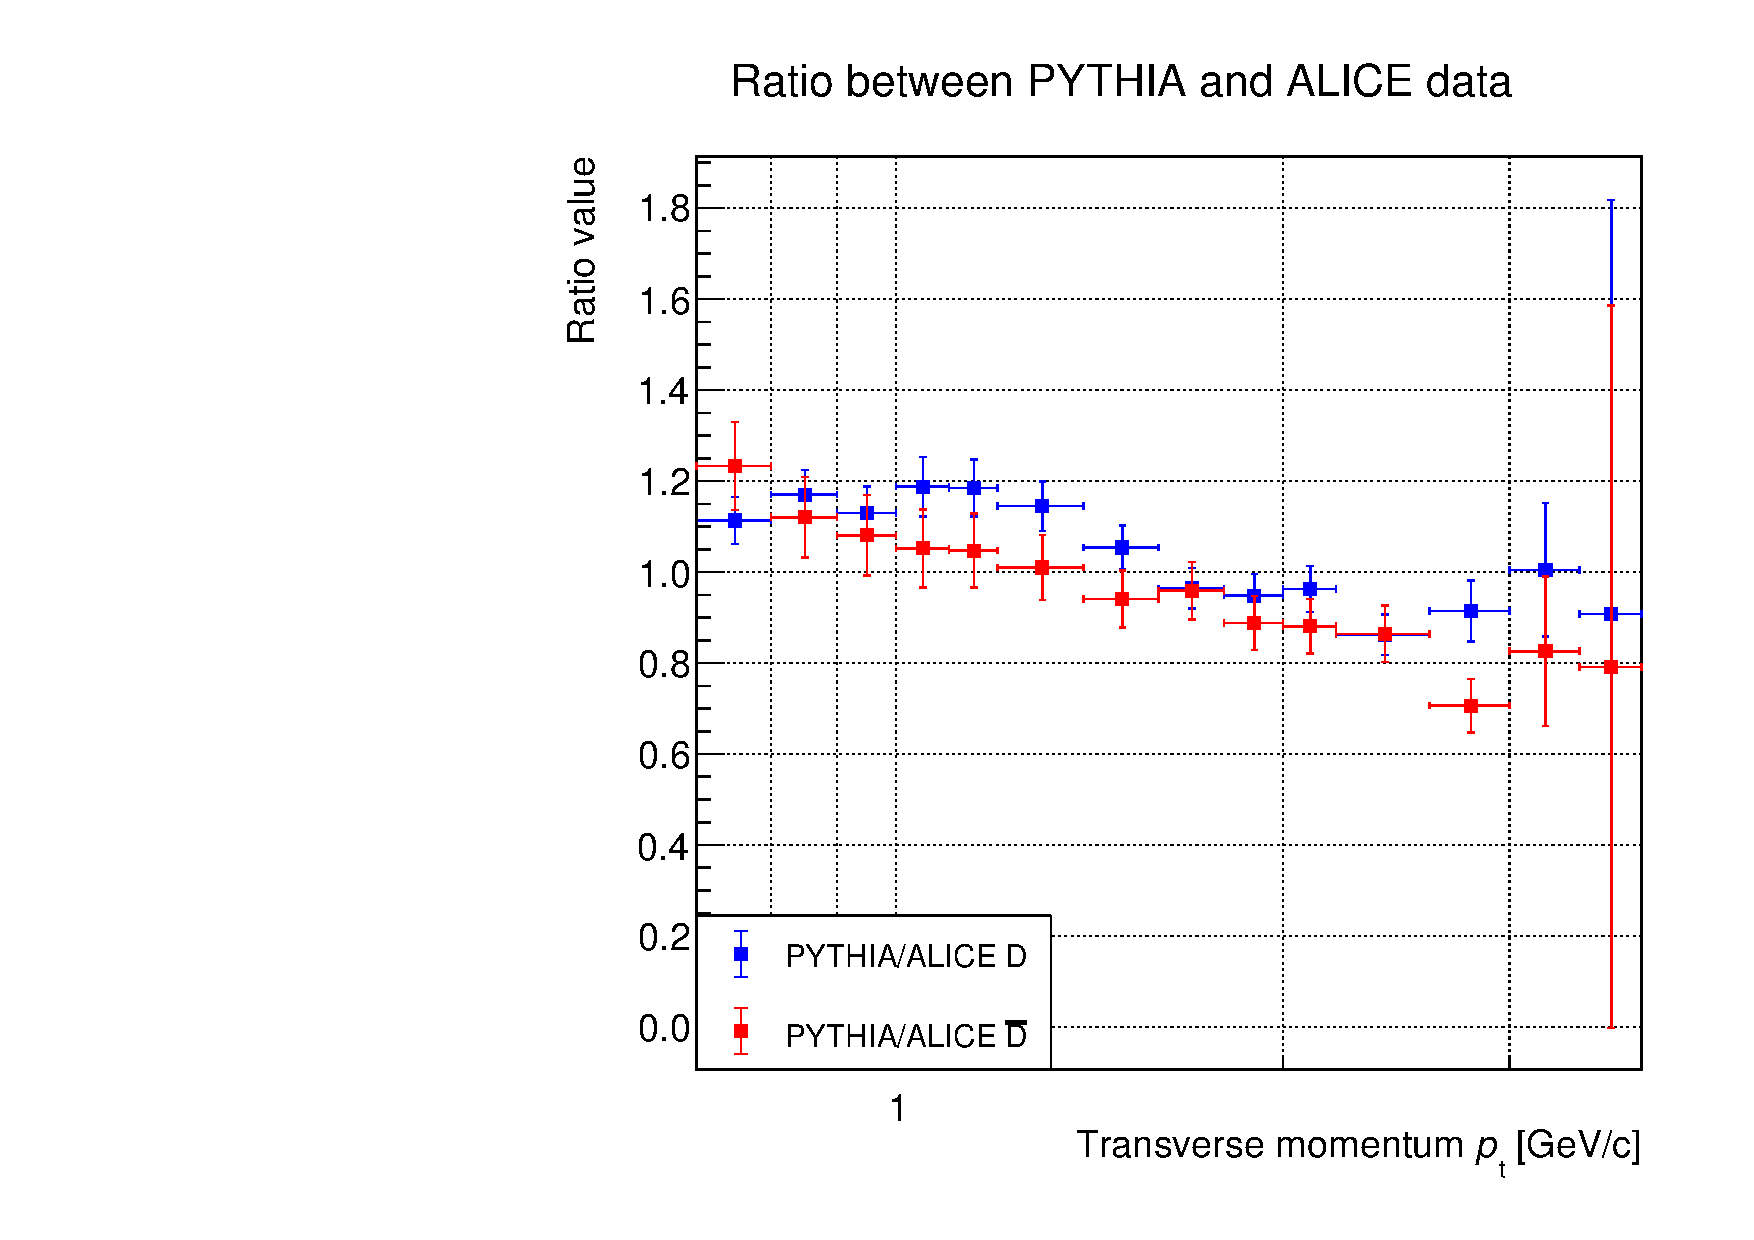
\includegraphics[width=\textwidth]{image/3-risultati/analyse/G/division.pdf}
        \caption{}
        \label{fig:D_division}
    \end{subfigure}
    %\hspace{1cm}
    \begin{subfigure}{.49\textwidth}
        \centering
        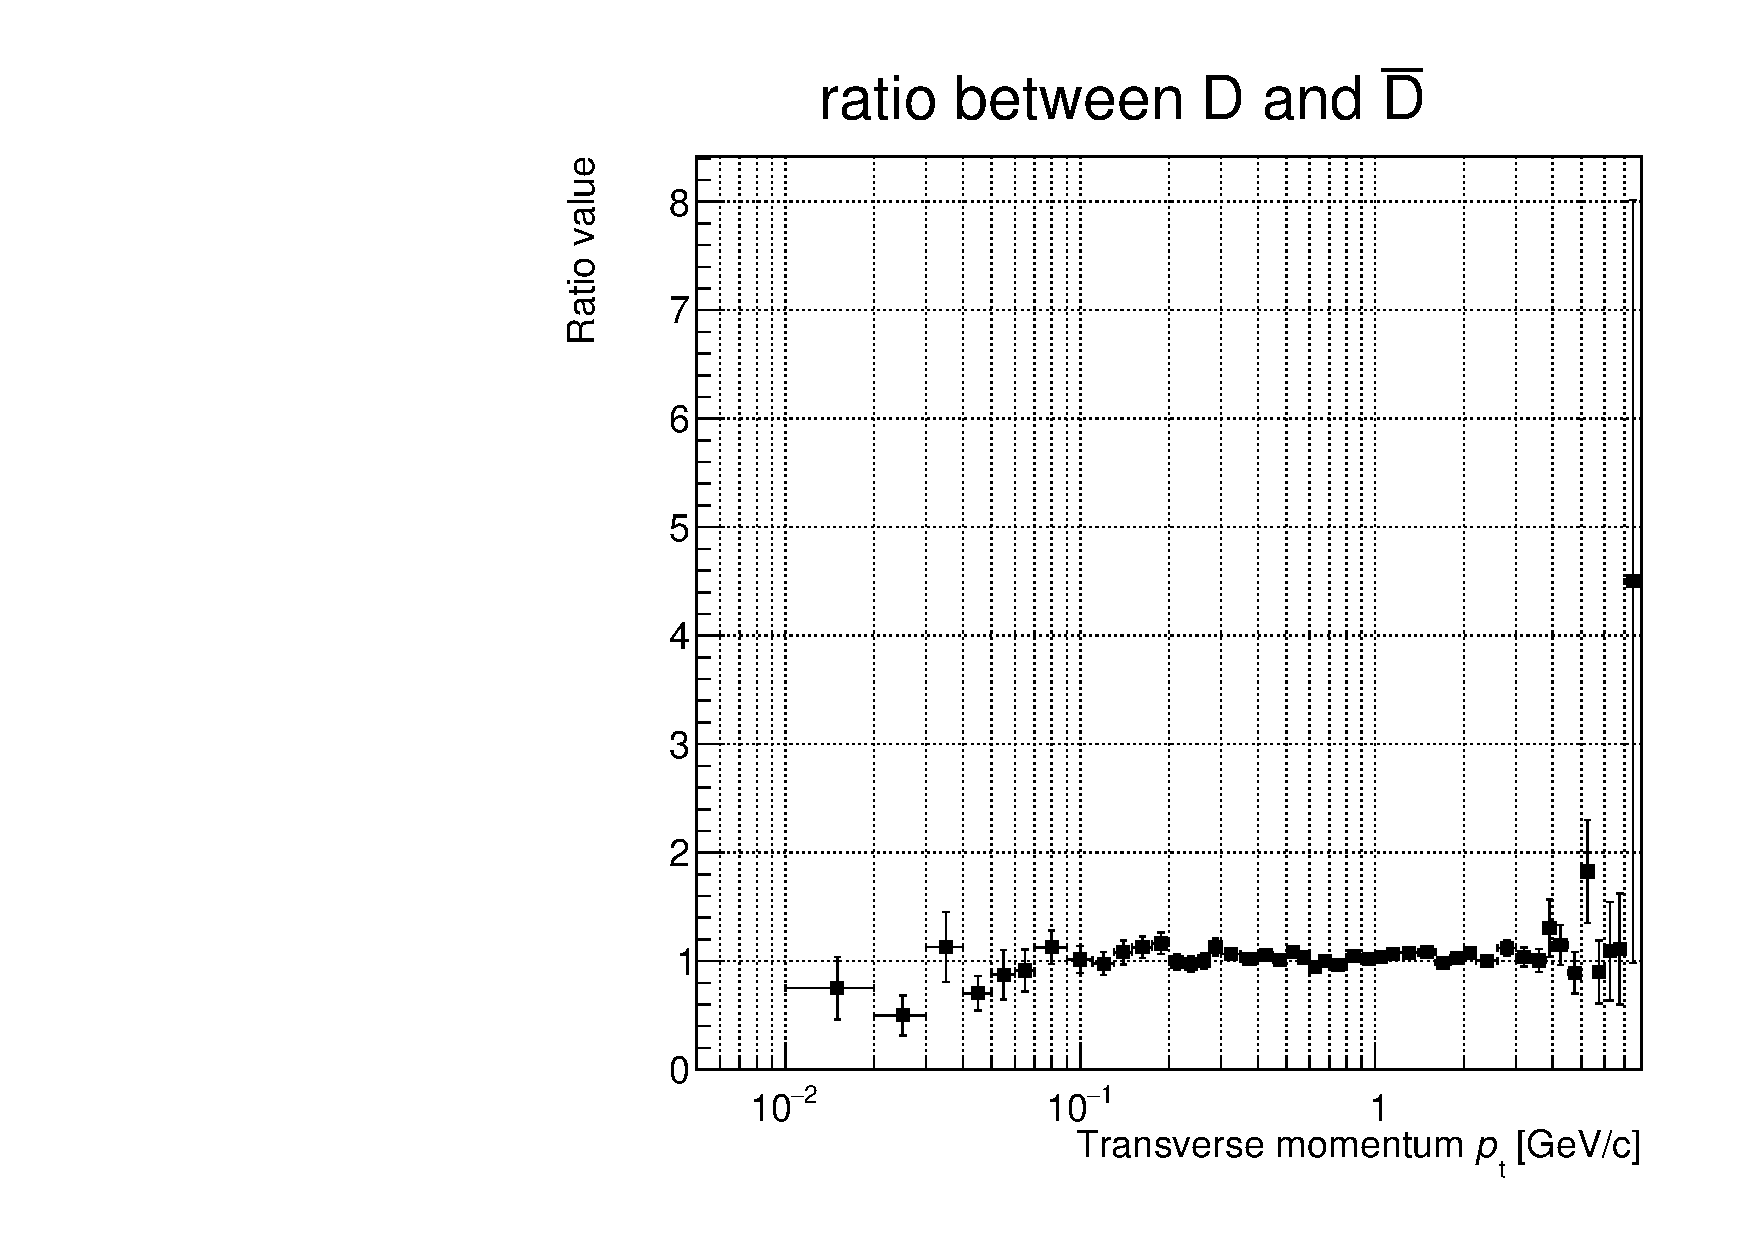
\includegraphics[width=\textwidth]{image/3-risultati/analyse/G/ratio_DD.pdf}
        \caption{}
        \label{fig:D_ratio_DD}
    \end{subfigure}
    \caption{\emph{\rmfamily (a)} Divisione tra la distribuzioni dell'impulso trasverso di $D$ e $\bar D$ con i dati di ALICE, utilizzando il modello ottimizzato. \emph{\rmfamily (b)} Frazione delle distribuzione dell'impulso trasverso di $D$ con quello di $\bar D$, utilizzando il modello ottimizzato.}
    \label{fig:D_ratio_DD_}
\end{figure}
\begin{figure}[h]
    \centering
    \begin{subfigure}{.49\textwidth}
    \centering
        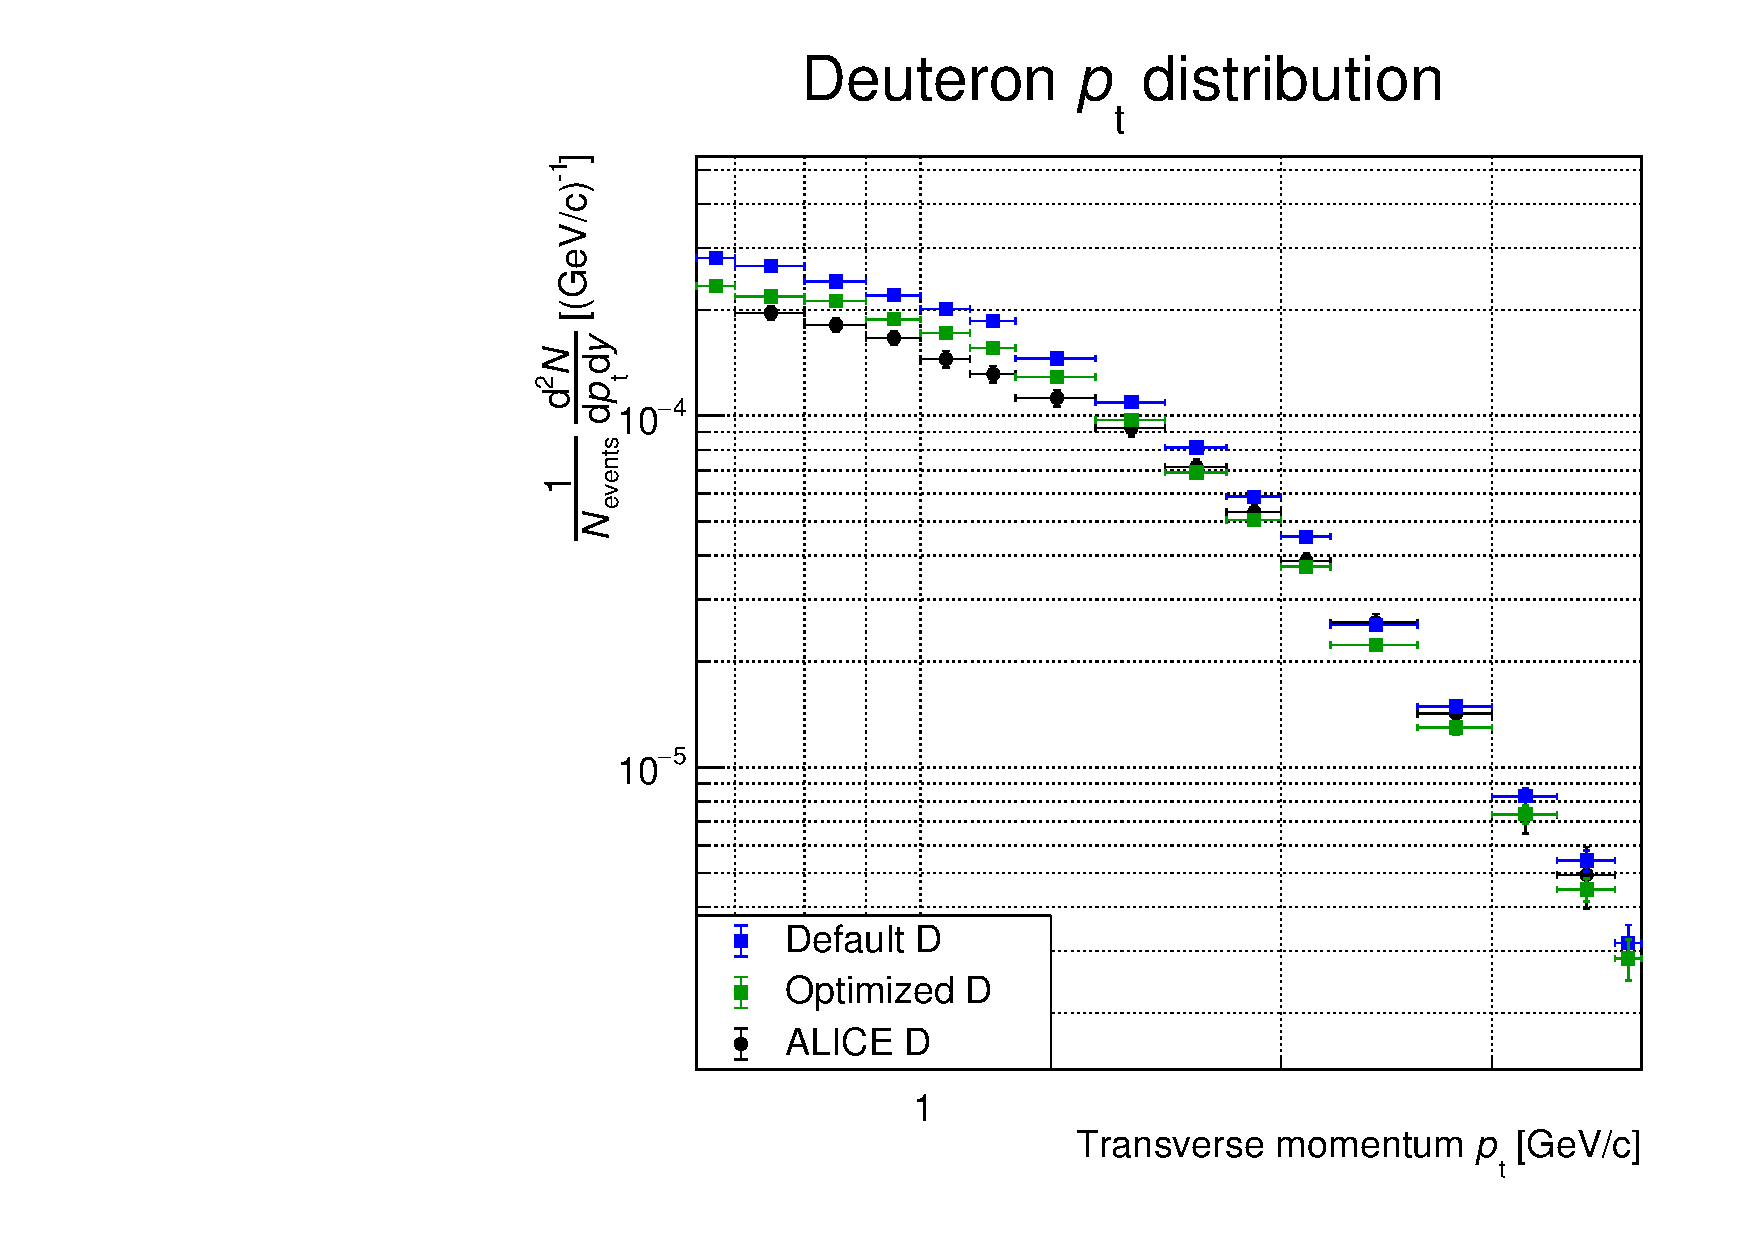
\includegraphics[width=\textwidth]{image/3-risultati/analyse/G/def_opt_deuteron.pdf}
        \caption{}
        \label{fig:def_opt_deuteron}
    \end{subfigure}
    %\hspace{1cm}
    \begin{subfigure}{.49\textwidth}
        \centering
        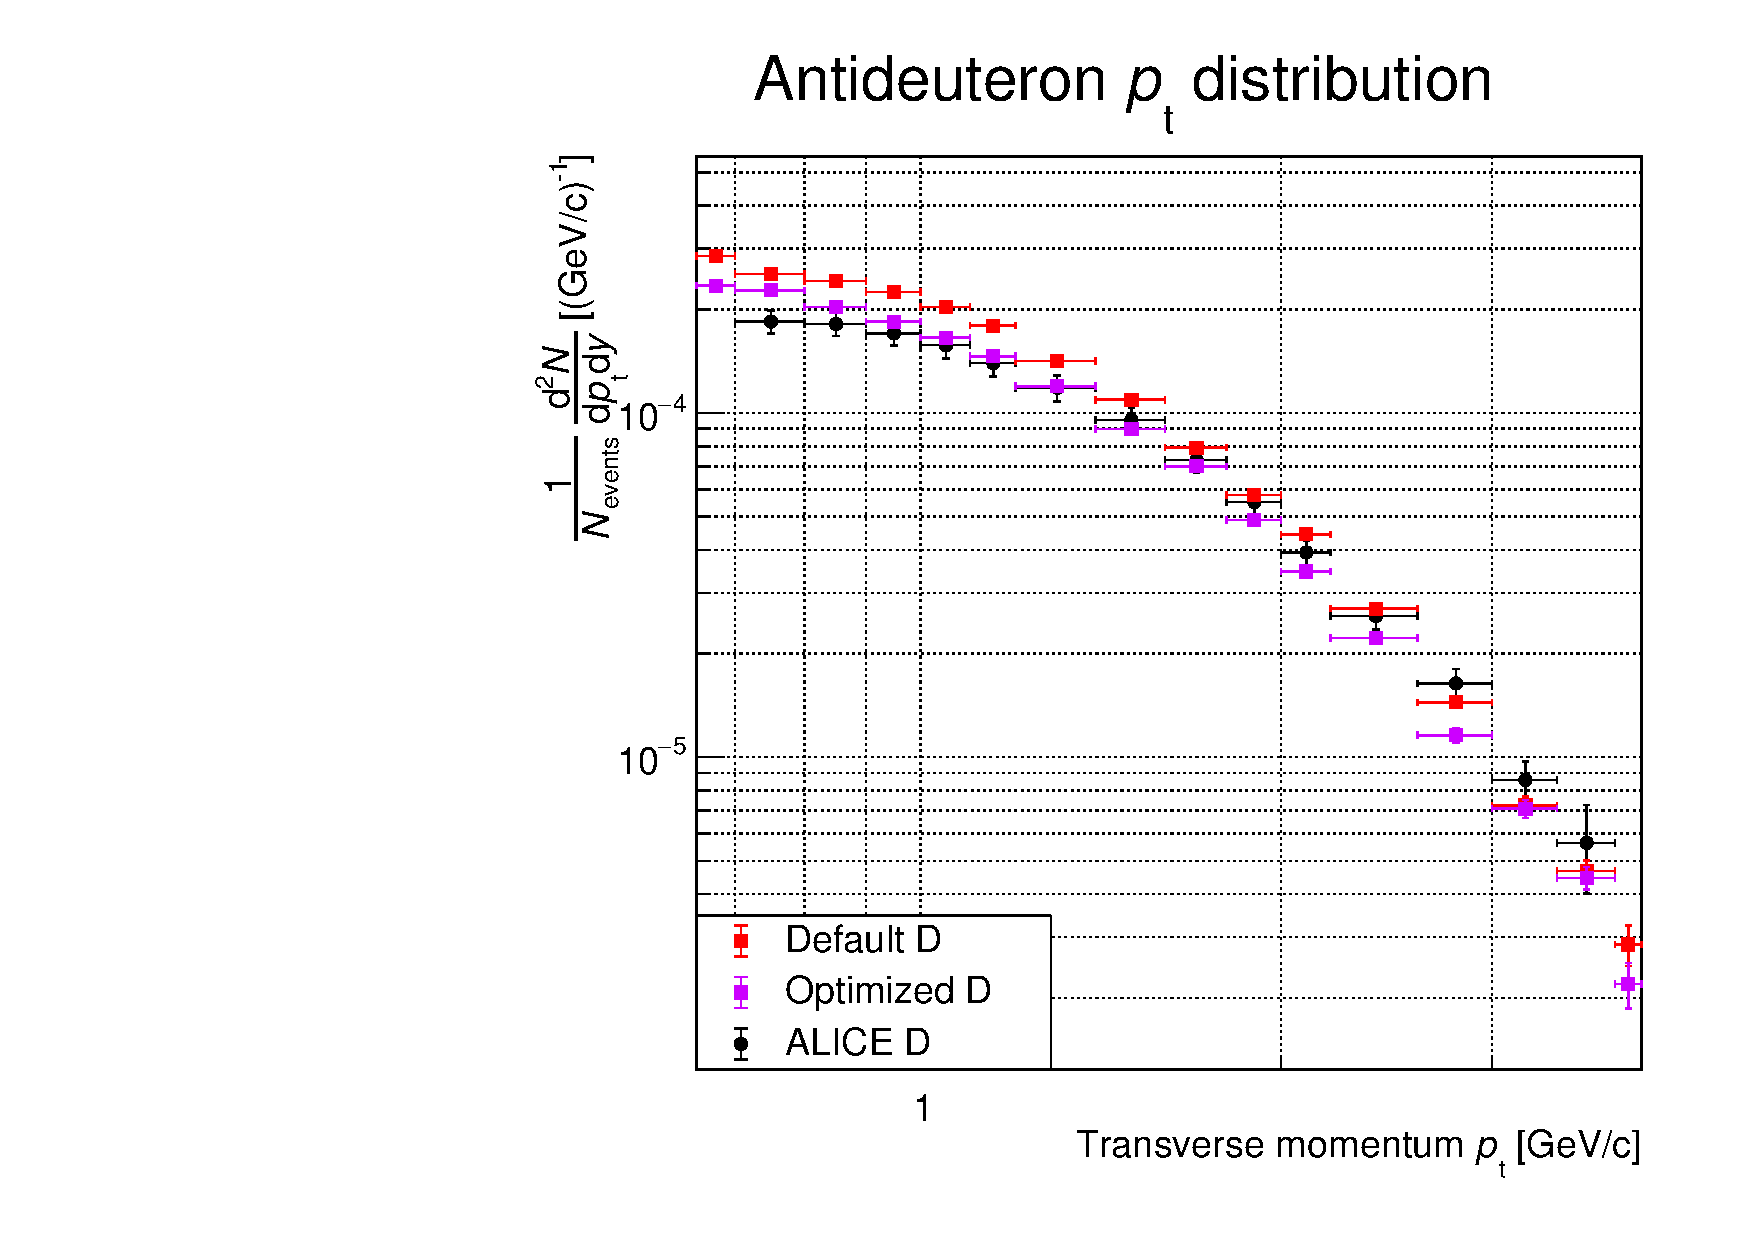
\includegraphics[width=\textwidth]{image/3-risultati/analyse/G/def_opt_antideuteron.pdf}
        \caption{}
        \label{fig:def_opt_antideuteron}
    \end{subfigure}
    \captionwithsource{Distribuzioni dell'impulso trasverso dei deuteroni e dei antideuteroni del modello predefinito ("Default"), ottimizzato ("Optimized") e dei dati di ALICE.}{\cite{ALICE:2020foi}} 
    \label{fig:def_opt}
\end{figure}